\documentclass{book}
\usepackage{hyperref} % For hyperlinks
\usepackage{fancyhdr}  % For customizing headers and footers
\usepackage{titlesec}  % For customizing title formats
\usepackage{inconsolata}
\usepackage[]{graphics} % For using local images
\usepackage{graphics} % For using local images
\usepackage{epstopdf}

\usepackage{color}
\definecolor{bluekeywords}{rgb}{0.13,0.13,1}
\definecolor{greencomments}{rgb}{0,0.5,0}
\definecolor{redstrings}{rgb}{0.9,0,0}

\usepackage{listings}
\lstset{language=[Sharp]C,
  showspaces=false,
  showtabs=false,
  breaklines=true,
  showstringspaces=false,
  breakatwhitespace=true,
  escapeinside={(*@}{@*)},
  commentstyle=\color{greencomments},
  keywordstyle=\color{bluekeywords},
  stringstyle=\color{redstrings},
  basicstyle=\ttfamily
}
\title{.NET Interview Questions}
\author{Konstantin Milchev }
\date{}

% Globally center all chapter titles
\titleformat{\chapter}[display]
  {\normalfont\huge\bfseries\centering} % Format for the chapter title (centering)
  {} % Label (empty since you may be using \chapter* for no numbering)
  {0pt} % Space before the title
  {\Huge} % Format of the chapter title itself

  
% Configure fancyhdr
\pagestyle{fancy}      % Use fancy page style for default layout
\fancyhf{}             % Clear all header and footer fields
\fancyfoot[C]{\thepage} % Set page number at the bottom center by default
\renewcommand{\headrulewidth}{0pt} % Remove the header line
\setlength{\headheight}{0pt}       % Remove the height of the header
 
\begin{document}

% Title Page
\maketitle

% Use \clearpage to avoid blank pages
\clearpage

% Table of Contents
\tableofcontents

% Start of the pages
 
\newpage
% Include other files here
\chapter{Patterns}
\input{Patterns/Prefix-Sum Pattern}
303, 525, 560

\chapter{Prefix - Suffix Product}
\section{Questions}\\


\href{https://leetcode.com/problems/product-of-array-except-self/description/}{238. Product of Array Except Self}


\section{Example Usage}\\



\begin{lstlisting}
 public int[] ProductExceptSelf(int[] nums) {
        var prefix = new int[nums.Length];
        var suffix = new int[nums.Length];
        var result = new int[nums.Length];

				prefix[0]=1;
        for(int i = 1; i<nums.Length; i++){
					prefix[i]=prefix[i-1]*nums[i-1];
        }


        suffix[nums.Length-1]=1;

        for(int j=nums.Length-2; j>= 0; j--){
            suffix[j]=suffix[j+1] * nums[j+1];
        }


        for(int i = 0; i<nums.Length; i++){
            result[i] = prefix[i]*suffix[i];
        }
        return result;
    }
		
\begin{figure}
		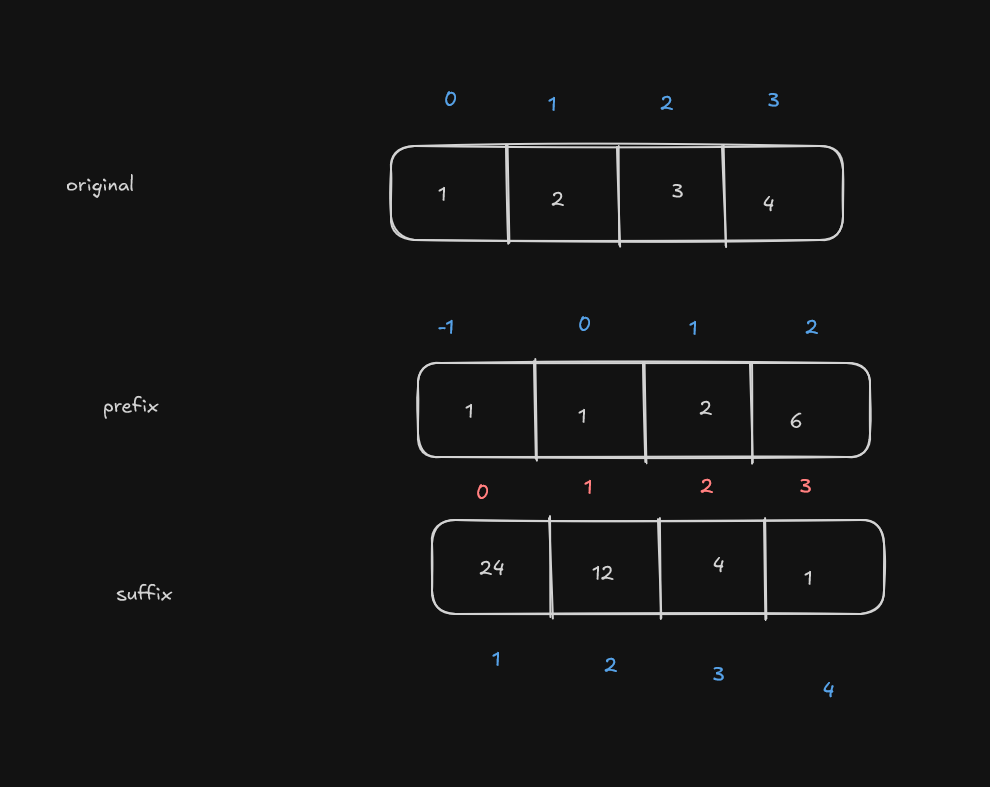
\includegraphics{1.png}
\end{figure}

\begin{figure}
		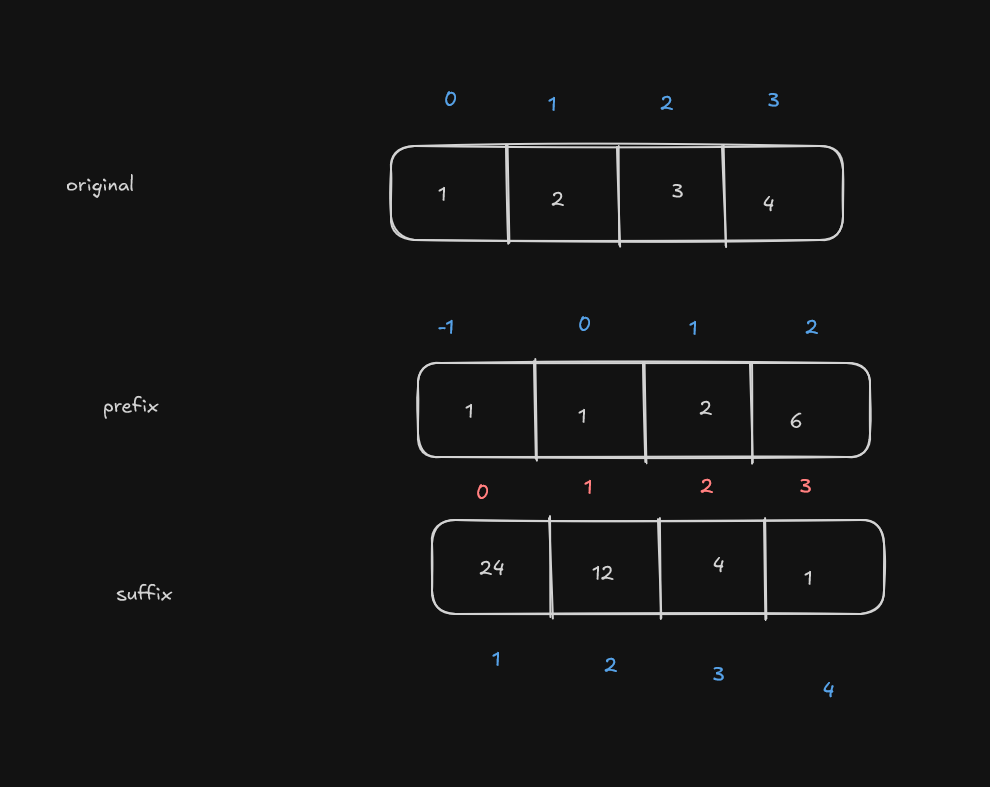
\includegraphics{1.eps}
\end{figure}

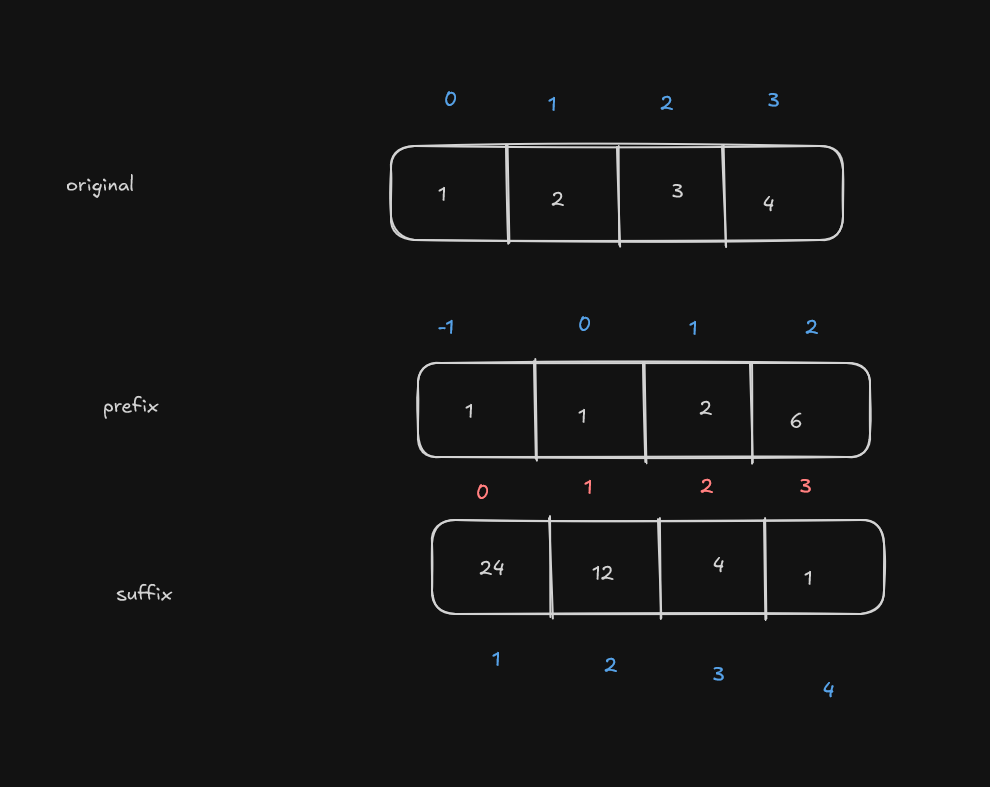
\includegraphics{1.eps}

\end{lstlisting}\\ \\


\chapter{Two Pointers}

\section{Explanation}

Having two pointers pointed at different parts of a string or an array. The pointers move from start and end closer to each other. Or they can move in the same direction

\section{When to use}
When we need to compare an element against other elements

\begin{itemize}
\item Comparing elements from two ends: Like checking for palindromes or finding pairs in a sorted array.
\item searching for a target sum or condition. In \textbf{"Two Sum"} where we need two numbers which meet a condition
\item Removing duplicates from sorted arrays
\item Finding subarrays like in \textbf{"Sliding Window"} problems
\end{itemize}	

\section{Example questions}
\begin{itemize}
\item Remove Duplicates From Sorted Array
\item Reverse String
\item Move Zeroes
\end{itemize}	
167, 15, 11


\include{Patterns/Fast and Slow Pointers}
141, 202, 287

\include{Patterns/Sliding Window} 
643, 3, 76

\include{Patterns/In-place Reversal of a LinkedList}
206, 92, 24

\include{Patterns/Monotonic Stack}
496, 739, 84


\include{Patterns/Top K Elements}
K Largest = Min - Heap
K Smallest = Max - Heap
215, 347, 373


\include{Patterns/Merge Intervals}
overlapping intervals
56, 57, 435

\section{Modified Binary Search}
\include{Patterns/Modified Binary Search}
33, 153, 240


\include{Patterns/Tree Breadth First Search}
102, 994, 127

\include{Patterns/Tree Depth First Search}
133, 113, 210

\include Binary Tree Traversal
257

InOrder
239

PostOrder
124

LevelOrder
107


\include{Patterns/Island}
733, 200, 130


\include{Patterns/Backtracking}
46, 78, 51

\include{Dynamic Programming}
COmmon Dp Patterns
1. Fibonaci Numbers
2. 0/1 Knapsack
3. Longest Common Subsequence
4. Longest Increasing Subsequence
5. Subset Sum
6. Matrix Chain Multiplication
70, 300, 322, 416, 1143, 312

\section{Cyclic Sort}
\include{Patterns/Cyclic Sort}

\section{Stack}
\chapter{Stack}

\section{Basics}
	\begin{itemize}
		\item Abstract data type that supports push and pop operations.
		\item Can be implemented using arrays and linked lists
		\item The behavior is often called LIFO( Last-In-First-Out)
		\item Used to implement \textbf{Depth-First-Search}
	\end{itemize}
	
	\section{Corner Cases}
		\begin{itemize}
			\item Empty stack. Popping from an empty stack
			\item Stack with one item
			\item Stack with two items
		\end{itemize}
		
	
	\section{Time complexity}
	
	\begin{center}
		\begin{tabular}{||c c||}
		\hline
		Operation & Complexity\\
		\hline\hline
		Top/Peek & O(1)\\
		\hline
		Push & O(1)\\
		\hline
		Pop & O(1)\\
		\hline
		isEmpty & O(1)\\
		\hline
		Search & O(n)\\
		\hline
			
		\end{tabular}
	\end{center}
	
	
	

\chapter{Hashmap}

\section{Questions}\\

Two Sum\\ \\
\href{https://leetcode.com/problems/two-sum/description/}{1. Two Sum}


\section{Example Usage}\\



\begin{lstlisting}
 public int[] TwoSum(int[] nums, int target)
 {
     var map = new Dictionary<int, int>();

     for (int i = 0; i < nums.Length; i++)
     {
         var diff = target - nums[i];
         if (map.ContainsKey(diff)) return [map[diff], i];
         map[nums[i]] = i;
     }
     throw new Exception();
 }
\end{lstlisting}\\ \\






\section{Graphs}
\include{Patterns/Graphs}



\section{Two Heaps}
\include{Patterns/Two Heaps}

\section{Subsets}
\include{Patterns/Subsets}



\section{Bitwise XOR}
\include{Patterns/Bitwise XOR}



\section{K-way Merge}
\include{Patterns/K-way Merge}


\chapter{Greedy Algorithm}

\section{Description}
A greedy algorithm makes an optimal choice at each step in the process, which then becomes the overall optimal choice.

\section{When to use}
A greedy algo can be implemented when some properties are in place
\begin{itemize}
\item Greedy Choice Property
	A global(overall) optimal solution can be reached by choosing the optimal choice at each step.
\end{itemize}

\section{Questions}

\href{https://leetcode.com/problems/best-time-to-buy-and-sell-stock/description/}{121. Best Time to Buy and Sell Stock}
 

 
\section{Example}

\begin{lstlisting}
 public int MaxProfit(int[] prices) {
var min = int.MaxValue;
var profit = 0;

    for(int i=0; i< prices.Length; i++){
        var currentProfit = prices[i] - min;
        profit = currentProfit > profit ? currentProfit: profit;

        min = min > prices[i] ? prices[i] : min;
    }
    return profit;
}
\end{lstlisting}







\section{Trie}
\include{Patterns/Trie}

\section{Topological Sort (Graph)}
\include{Patterns/Topological Sort}

\section{Union Find}
\include{Patterns/Union Find}

\section{Ordered Set}
\include{Patterns/Ordered Set}

\section{Multi-thread}
\include{Patterns/Multi-thread}


\chapter{Data Structures}

\chapter{Array}

\section{Definition}
\begin{itemize}
	\item Arrays hold values of the same type of data at contiguous memory locations.
\end{itemize}

\section{Advantages}
\begin{itemize}
	\item Store multiple elements of the same type in one variable name.
	\item Accessing elements is fast if the index is known.
\end{itemize}

\section{Disadvantages}
\begin{itemize}
	\item Removing/Adding from the middle or start of the array is slow because other elements need to be moved around.
\end{itemize}

\section{Corner Cases}
\begin{itemize}
	\item Empty Sequence
	\item Sequence with 1 or 2 elements
	\item Sequence with repeated elements
	\item Duplicated values in the sequence
\end{itemize}

\begin{center}
\begin{tabular}{||c c||} 
 \hline
 Operation & Complexity\\ [0.5ex] 
 \hline\hline
 Access & O(1) \\ 
 \hline
 Search & O(n) \\
 \hline
 Seach(sorted) & \[O(\log(n))\] \\
 \hline
 Insert & O(n) \\
 \hline
 Insert(at end) & O(1)\\ [1ex] 
 \hline
 Remove & O(n) \\ [1ex] 
 \hline
 Remove(at end) & O(1) \\ [1ex] 
 \hline

\end{tabular}
\end{center}
\include{DataStructures/String}
\chapter{Hashmap}

\section{Questions}\\

Two Sum\\ \\
\href{https://leetcode.com/problems/two-sum/description/}{1. Two Sum}


\section{Example Usage}\\



\begin{lstlisting}
 public int[] TwoSum(int[] nums, int target)
 {
     var map = new Dictionary<int, int>();

     for (int i = 0; i < nums.Length; i++)
     {
         var diff = target - nums[i];
         if (map.ContainsKey(diff)) return [map[diff], i];
         map[nums[i]] = i;
     }
     throw new Exception();
 }
\end{lstlisting}\\ \\



\chapter{Recursion}
\section{Definition}
Recursion is a method of solving a computational problem where the solution depends on solutions to smaller instances of the same problem.
\section{Basics}
	\begin{itemize}
		\item Steps of a recursive function
			\begin{itemize}
			\item Base Case (i.e. when to stop)
			\item Work toward Base Case
			\item Recursive Call
			\end{itemize}
		\begin{lstlisting}
def fib(n):
	if n <= 1:
    return n
  return fib(n - 1) + fib(n - 2)
	\end{lstlisting}
	\end{itemize}
	
	\section{Corner Cases}
\begin{itemize}
	\item n = 0
	\item n = 1
\end{itemize}

		
		\section{Techniques}
		\begin{itemize}
			\item \textbf{Memoization}
			Memoization is an optimization technique which stores the results of expensive function calls and reuses them when the same inputs occur again.
		\begin{itemize}
			\item If you see a top or lowest k being mentioned in the question, it is usually a signal that a heap can be used to solve the problem, such as in \textbf{Top K Frequent Elements.}
			\item Stack with one item
			\item Stack with two items
		\end{itemize}
		\end{itemize}


\include{DataStructures/SortingAndSearching}
\include{DataStructures/Matrix}
\chapter{Array}

\section{Definition}
\begin{itemize}
	\item Like arrays it's used to represent sequential data.
	\item Each element contains an address of the next element.
	\item A collection of nodes where each node contains data and a reference to the next node in the sequence.
\end{itemize}

\section{Advantages}
\begin{itemize}
	\item Deletion and Insertion of a node given it's location is constant O(1), where in arrays the items would have to be shifted.
\end{itemize}

\section{Disadvantages}
\begin{itemize}
	\item Accessing a node is linear time O(n).
	\item Accessing can only occur by traversing from the head. Access by index (as with arrays) not possible.
\end{itemize}

\section{Types}
\begin{itemize}
	\item Singly Linked List
			\begin{itemize}
				\item Each node points to the next node and the last node points to null.
			\end{itemize}
	\item Doubly Linked List
			\begin{itemize}
				\item Each node has two pointers. Next and Prev.
				\item The first node's Prev and the last node's Next pointers point to null.
			\end{itemize}
\end{itemize}

\section{Corner Cases}
\begin{itemize}
	\item Empty Sequence
	\item Sequence with 1 or 2 elements
	\item Sequence with repeated elements
	\item Duplicated values in the sequence
\end{itemize}

\begin{center}
\begin{tabular}{||c c c||} 
 \hline
 Operation & Complexity & Note\\ [0.5ex] 
 \hline\hline
 Access & O(n) \\ 
 \hline
 Search & O(n) \\
 \hline
 Insert & O(1) & Assumes you have traversed to the insertion position \\ 
 \hline
 Remove & O(1) & Assumes you have traversed to the node to be removed \\
 \hline

\end{tabular}
\end{center}

\section{Common Routines to Remember}
\begin{itemize}
	\item Counting the number of nodes in the linked list
	\item Reversing a linked list in-place
	\item Finding the middle node of the linked list using two pointers (fast/slow)
	\item Duplicated values in the sequence
\end{itemize}


\section{Corner Cases}
\begin{itemize}
	\item Empty linked list (head is null)
	\item Single node
	\item Two nodes
	\item Linked list has cycles. Tip: Clarify beforehand with the interviewer whether there can be a cycle in the list. Usually the answer is no and you don't have to handle it in the code
\end{itemize}
\include{DataStructures/Queue}
\chapter{Stack}

\section{Basics}
	\begin{itemize}
		\item Abstract data type that supports push and pop operations.
		\item Can be implemented using arrays and linked lists
		\item The behavior is often called LIFO( Last-In-First-Out)
		\item Used to implement \textbf{Depth-First-Search}
	\end{itemize}
	
	\section{Corner Cases}
		\begin{itemize}
			\item Empty stack. Popping from an empty stack
			\item Stack with one item
			\item Stack with two items
		\end{itemize}
		
	
	\section{Time complexity}
	
	\begin{center}
		\begin{tabular}{||c c||}
		\hline
		Operation & Complexity\\
		\hline\hline
		Top/Peek & O(1)\\
		\hline
		Push & O(1)\\
		\hline
		Pop & O(1)\\
		\hline
		isEmpty & O(1)\\
		\hline
		Search & O(n)\\
		\hline
			
		\end{tabular}
	\end{center}
	
	
	
\include{DataStructures/Tree}
\include{DataStructures/Graph}
\chapter{Heap}
\section{Definition}
	A heap is a \textbf{binary} tree with two properties:
	\begin{itemize}
		\item Shape: Its shape must be complete. All of the nodes from all the levels must be filled, except the last one.
		\item Order: It must have all of its nodes in a specific order.
		\begin{itemize}
			\item \textbf{Min-Heap}: A heap's root node must have of its children be either smaller than or equal to it's children.
			\item \textbf{Max-Heap}: A heap's root node must have of its children be either greater than or equal to it's children.
		\end{itemize}
	\end{itemize}
\section{Basics}
	\begin{itemize}
		\item We can always have duplicates in a heap
		\item Heaps don't follow the binary search tree rule that the left node needs to be smaller than the right.
		\item No matter if we grow or shrink the heap, we must always maintain it's two properties
		\item It's used in a system scheduler where a priority queue will say which task should be executed next (task, item with highest priority will be dequeued from the heap)
	\end{itemize}
	\section{Storing a Heap}
	\begin{figure}[H]
		\centering
		\scalebox{0.40}
			{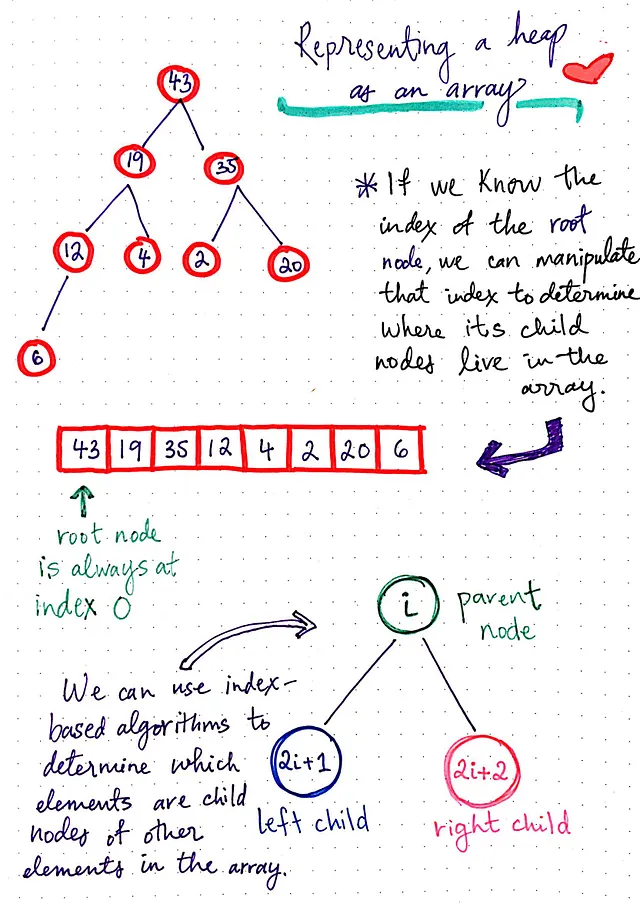
\includegraphics{images/heap_1}}
		\caption{Heap as an array structure}
	\end{figure}	
	
	\section{Getting the heap out of the Array}
	\begin{figure}[H]
		\centering
		\scalebox{0.40}
			{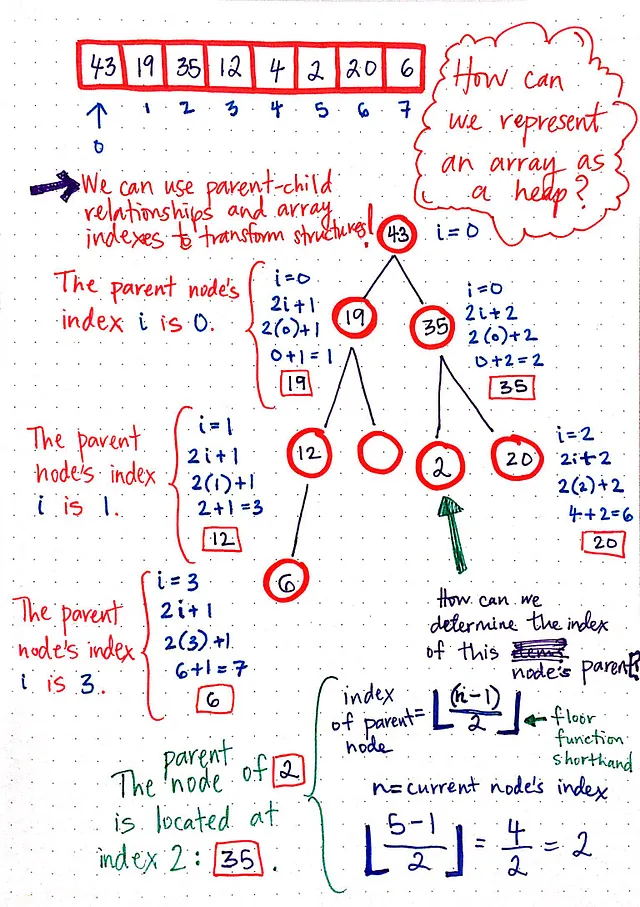
\includegraphics{images/heap_2}}
		\caption{Heap as an array structure}
	\end{figure}	
	
	\section{Heap Sort Algorithm}
		\begin{itemize}
			\item Improved Selection Sort with O(nlogn) time complexity
			\item buildMaxHeap()
			\item heapify()
		\end{itemize}

		
		\section{Techniques}
		\begin{itemize}
			\item If you see a top or lowest k being mentioned in the question, it is usually a signal that a heap can be used to solve the problem, such as in \textbf{Top K Frequent Elements.}
			\item Stack with one item
			\item Stack with two items
		\end{itemize}
		
	
	\section{Time complexity}
	
	\begin{center}
		\begin{tabular}{||c c||}
		\hline
		Operation & Complexity\\
		\hline\hline
		Find max/min & O(1)\\
		\hline
		Insert & O(log(n))\\
		\hline
		Remove & O(log(n))\\
		\hline
		Heapify(create a heap of a given array of elements) & O(1)\\
		\hline
			
		\end{tabular}
	\end{center}
	
	
	
\include{DataStructures/Trie}
\include{DataStructures/Interval}
\include{DataStructures/DynamicProgramming}
\include{DataStructures/Binary}
\include{DataStructures/Math}
\include{DataStructures/Geometry}

	


\end{document}
